% Poss�veis TODO
% - linkar as se��es de pesq � se��o hist�rica
\documentclass[a4paper,titlepage]{article}
\usepackage[latin1]{inputenc}
\usepackage[T1]{fontenc}
\usepackage[portuges]{babel}
% setspace - \doublespace \onehalfspace
% fullpage - ??
\usepackage{verbatim,url}
\usepackage[dvips]{graphicx}
\usepackage[bf]{subfigure}
\usepackage[bf]{caption}
\usepackage{amsmath, amssymb, algorithm, algorithmic,fullpage,setspace}
\usepackage{mathtools,empheq}
\usepackage[pagebackref=true,breaklinks=true,letterpaper=true,colorlinks,bookmarks=false]{hyperref}
\usepackage{multirow}
\usepackage{xspace}
\usepackage{array}

\newtheorem{definition}{Defini��o}
\newtheorem{theorem}{Teorema}
\newtheorem{notation}{Nota��o}
\floatname{algorithm}{Algoritmo}

\newenvironment{changemargin}[2]{\begin{list}{}{
   \setlength{\topsep}{0pt}\setlength{\leftmargin}{0pt}
   \setlength{\rightmargin}{0pt}
   \setlength{\listparindent}{\parindent}
   \setlength{\itemindent}{\parindent} \setlength{\parsep}{0pt plus 1pt}
   \addtolength{\leftmargin}{#1}\addtolength{\rightmargin}{#2}
}\item }{\end{list}}

%%%%%%%%%%%%%%%%%%%%%%%%%%%%%%%%%%%%%%%%
% You have many versions of the macro \draftnote{My note}. 
% The first version puts notes (My note in the example)
% into the margin. The others insert within the document. 
% Toggle the empty definitions to hide all draft notes.

\newcommand{\draftnote}[1]{\marginpar{\tiny\raggedright\textsf{\hspace{0pt}#1}}}
%\newcommand{\draftnote}[1]{}
%
% This one is just for the comments for in-line text.
\newcommand{\indraftnote}[1]{\textcolor{blue}{\texttt{\footnotesize [#1]}}}
%\newcommand{\indraftnote}[1]{}

\newcommand{\todo}[1]{\indraftnote{todo: #1}}
%\newcommand{\todo}[1]{}
\usepackage{listings} % better verbatim env for sketching outlines/lists
\lstset{
basicstyle=\small,
columns=flexible,
breaklines=true
}

% Uncomment to eliminate draft text
\lstnewenvironment{draft}{ } { }
%\newenvironment{draft} {\expandafter\comment} {\expandafter\endcomment}   % Empty 

\newcommand{\scilab}{\textsc{Scilab}}
\newcommand{\matlab}{\textsc{Matlab}}
\newcommand{\sip}{SIP}
\newcommand{\animal}{AnImaL}
\newcommand{\eg}{{p.\ ex.}}
\newcommand{\etc}{{\it etc}}
\newcommand{\ie}{{\it i.e.}}
\newcommand{\etal}{{\it et al.}}
\newcommand{\id}{\text{\emph{Id}}}
\newcommand{\dof}{\textsc{dof}}
\newcommand{\ransac}{\textsc{ransac}}
\newcommand{\sift}{\textsc{sift}}
\newcommand{\svd}{\textsc{svd}}
\newcommand{\sfm}{\textsc{sfm}}

\newcommand{\Gama}{\boldsymbol{\Gamma}}
\newcommand{\gama}{\boldsymbol{\gamma}}
\newcommand{\bsigma}{\boldsymbol{\sigma}}
%\newcommand{\Gama}{\Gamma}
%\newcommand{\gama}{\gamma}
\newcommand{\T}{\boldsymbol{T}}
\newcommand{\N}{\mathbf{N}}
\newcommand{\NSurface}{\mathbf{N}}
\newcommand{\Nlocal}{\overline{\N}} % normal in local coordinates
\newcommand{\balpha}{\boldsymbol{\alpha}}
\newcommand{\tDt}{t+\Delta t}
\newcommand{\bpsi}{\boldsymbol{\boldsymbol{\psi}}}
\newcommand{\bp}{\mathbf p}
\newcommand{\deldt}[1]{\frac{\partial#1}{\partial t}}
\newcommand{\ddt}[1]{\frac{d #1}{dt}}
\newcommand{\delds}[1]{\frac{\partial#1}{\partial s}}
\newcommand{\mybar}[1]{\overline{#1}}
\newcommand{\norm}[1]{\|#1\|}
\newcommand{\I}{\mathbf{I}}
\newcommand{\brho}{\boldsymbol{\rho}}
\newcommand{\lightrgb}{\boldsymbol{l}}
\newcommand{\B}{\boldsymbol{B}}
\renewcommand{\t}{\boldsymbol{t}}
\newcommand{\n}{\boldsymbol{n}}
\renewcommand{\b}{\boldsymbol{b}}
\newcommand{\e}{\boldsymbol{e}}
\newcommand{\f}{\boldsymbol{e}_3}
\newcommand{\ff}{\mathbf{f}}
\newcommand{\hf}{\boldsymbol{\hat{f}}}
\newcommand{\g}{\boldsymbol{g}}
\newcommand{\G}{\boldsymbol{G}}
\newcommand{\bc}{\boldsymbol{c}}
\newcommand{\Curve}{\Gamma}
%\newcommand{\X}{\boldsymbol{X}}
%\newcommand{\x}{\boldsymbol{x}}
\newcommand{\X}{\mathbf{X}}
\newcommand{\x}{\mathbf{x}}
\newcommand{\tilx}{\tilde x}
\newcommand{\tily}{\tilde y}
\newcommand{\tilgama}{\tilde \gama}
\newcommand{\ugama}{\hat{\gama}} %unit gama
\newcommand{\br}{\bar r}
\newcommand{\Kc}{\mathbf K_c}
\newcommand{\Kim} {\mathcal K_{im}}
\newcommand{\lepi}{\mathbf r}
\newcommand{\itan}{\tan^{-1}}
\newcommand{\uu}{\xi}
\newcommand{\buu}{\bar \uu}
\newcommand{\bvv}{\bar \vv}
\newcommand{\vv}{\eta}
\newcommand{\VV}{\mathbf{V}} % translational velocity
\newcommand{\VVspeed}{V} % translational velocity
\newcommand{\field}{\boldsymbol\chi}
\newcommand{\ufield}{\hat{\boldsymbol{\chi}}}
\newcommand{\fieldc}{\chi} % field component
\newcommand{\transl}{\mathcal{T}}
\newcommand{\rot}{\mathcal{R}}
\newcommand{\albedo}{\alpha}
\newcommand{\depth}{\rho}      % depth as z
\newcommand{\udepth}{{\hat{\rho}}} % depth along ray
\newcommand{\ttransl}{\T} % translation tangent
\newcommand{\surface}{\mathcal{M}} % surface/manifold
\newcommand{\surf}{\mathcal{M}} % surface/manifold short
\newcommand{\jacm}{\mathtt{J}} % Jacobian matrix
\newcommand{\xbar}{\bar x}
\newcommand{\ybar}{\bar y}
\newcommand{\zbar}{\bar z}

\newcommand{\bdelta}{\boldsymbol \delta}
%\newcommand{\X}{\boldsymbol{X}}
%\newcommand{\x}{\boldsymbol{x}}
%\newcommand{\X}{\mathbf{X}}
%\newcommand{\x}{\mathbf{x}}
\newcommand{\boldu}{\mathbf{u}}
\newcommand{\boldv}{\mathbf{v}}
\newcommand{\boldw}{\mathbf{w}}
\newcommand{\tgtveloc}{\tilde\alpha} % real tangential velocity
\newcommand{\mccn}{\textsc{mccn}\xspace}

\newcommand{\argmin}{\operatornamewithlimits{argmin}}
\newcommand{\argmax}{\operatornamewithlimits{argmax}}
\newcommand{\avg}{\operatornamewithlimits{avg}}

\begin{document}

\begin{titlepage}
\begin{changemargin}{-0.5cm}{-1cm}
\renewcommand{\title}{%
  {\LARGE Assinaturas de Sinais Geométricos}\\[4pt]
  {\LARGE para Reconstrução 3D Multiperspectiva de Curvas e Superfícies}
}
\renewcommand{\author}{Clêuber Eduardo do Nascimento Silva}
%\renewcommand{\date}{\today}
\newcommand{\info}{%
  \raisebox{4pt}[-4pt]{%
  
\includegraphics[height=1.3cm]{figs/logo-iprj2.eps} 
  \hspace{0.1in}
  }

  Laboratório de Visualização\\
  Laboratório de Tecnologia da Informação\\
  Instituto Politécnico -- IPRJ\\
  Universidade do Estado do Rio de Janeiro\\[1.5cm]

  Nova Friburgo, 15 de Novembro de 2020\\[1.5cm]

  \textbf{Projetos Relacionados}\\[4pt]
   FAPERJ Jovem Cientista do Nosso Estado E25/2014 204167\\
   FAPERJ APQ1 01/09335-8\\
   FAPERJ E28/2014/204747\\
   UERJ Prociência 2014--2017
}

%% Abstand zwischen oberem Blattrand und Titel.
\newlength{\topToTitle} 
\setlength{\topToTitle}{30pt}

%% Abstand zwischen linkem Blattrand und Titel.
\newlength{\leftToTitle} 
\setlength{\leftToTitle}{-50pt}

%% Abstand zwischen Titel und Info-Feld.
\newlength{\titleToInfo} 
\setlength{\titleToInfo}{7cm}

%% \myTextWidth erhoehen, um Info-Feld weiter nach Rechts zu schieben.
\newlength{\myTextWidth}
\setlength{\myTextWidth}{\textwidth}
\advance\myTextWidth by 1.5cm


\thispagestyle{empty}
\vspace*{\topToTitle}
\begin{minipage}{\myTextWidth}
  \sffamily
  \hspace*{\leftToTitle}\begin{minipage}{60cm}
    \Large\textbf{Plano de Trabalho de Doutorado}\\[1.5cm]
    \title\\[1.5cm]
    \author
  \end{minipage}\\

  %% \enlargethispage{} um ggfs. Titel und Info-Feld weiter
  %% auseinanderziehen zu koennen.
  \vspace*{\titleToInfo}

  \begin{minipage}{\textwidth}
    \flushright
    \info
  \end{minipage}
\end{minipage}%
\end{changemargin}
\end{titlepage}


%\tableofcontents
%\contentsline {section}{Refer\^{e}ncias}{16}
%\newpage
%\doublespacing
%\onehalfspacing
%

%%%%%%%%%%%%%%%%%%%%%%%%%%%%%%%%%%%%%%%%%%%%%%%%%%%
% TODO  TODO TODO 
%  - italico em spots e sub-arrays
%  - XXX
%  - @@@
%%%%%%%%%%%%%%%%%%%%%%%%%%%%%%%%%%%%%%%%%%%%%%%%%%% 


TODO
\begin{itemize}
\item Include prev projects for book
\item Think: how to make nonlinear reconstruction useful here
\item Recall my hand notes on this
\item Bring in whatever is useful from NSF prop.
\item Photos I had taken from whiteboard with Ben in 2018
\end{itemize}

\section{Introduction and Context}

\begin{itemize}
\item Explain my prev work both in 3D and machine learning/diffusion
\item Explain that to mak
\item Midlevel semantic representation, along lines of NSF
\end{itemize}

\begin{draft}
  [figure of usual reconstruction problem]
  [figure of loft surface]
  [figure of pipelines] - say we are working on the surface pipelines
\end{draft}

\begin{figure*}
  \begin{center}
    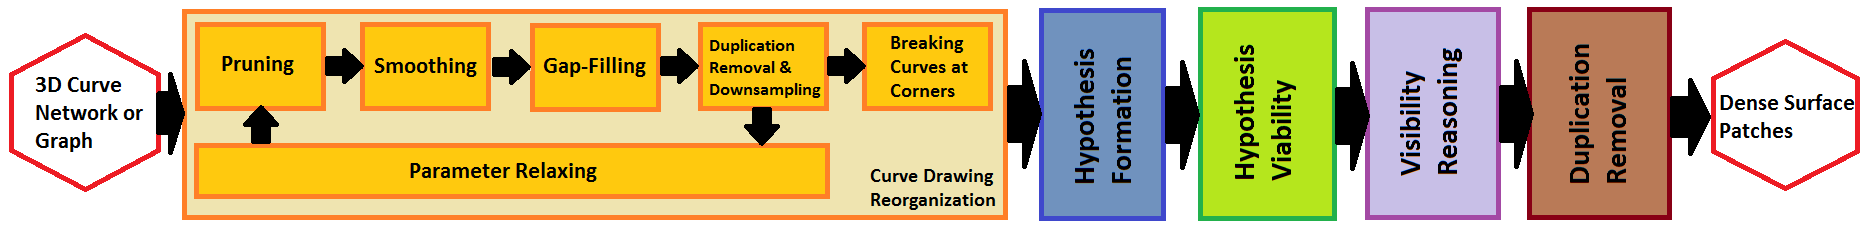
\includegraphics[width=\linewidth]{figs/lofting-pipeline.png}
  \end{center}
%  \ReduceBeforeCaptionfigspace
  \caption{A visual illustration of our dense surface reconstruction pipeline.
  }
%  \ReduceAfterCaptionfigspace
  \label{fig:lofting:pipeline}
\end{figure*}

\section{Objectives}

\subsection{Optimal view-selection}
\begin{itemize}
\item What views to use to perform a fine-grain 3D reconstruction, once a
  coarse initial reconstruction is available?
\item If we are going to do the 3D rec from drawing progressively, what are the
  next views to use to get more info?
\end{itemize}

\subsection{Finding Patterns in 2D-3D Networks}

\begin{itemize}
\item Main goal: better surface patches
\item Explain my 3D curve graphs
\item How to figure out if a cloud of points + curve fragments are volumetric or
  not, and if so, can we perform the next stage of reconstruction there?
\item How to do better than meshing 3D points, using both the image info and the
  curve info.
\item Can we start a graph between the pairwise surface patches, and use that
  graph to figure out which patches to merge?
\item Include graphs here.
\end{itemize}

\textbf{Multiview Local Consistency Network:}
The key idea underlying integration of reconstructions across views is the
detection of a common image structure supporting two reconstruction hypotheses. 
Two 3D local curve segments depict the same single underlying
3D object feature if they are supported by the same 2D image edge structures. 
Since the identification of common image structure can vary along the curve, it
must necessarily be a local process, operating at the level of a 3D local edge
and not a 3D curve. 
Two 3D edge elements (edgels) depict the same 3D structure if they 
receive support from the same 2D edgels in a sufficient number of views, so
3D-2D links between a 2D edgel to the 3D edgel it supports must be kept. Typically,
they share supporting image edges in many views; and the number of shared
supporting edgels is the measure of strength for a 3D-3D link between them.

Formally, we define the Multiview Local
geometric consistency Network (MLN) as pointwise alignments $\phi_{ij}$ between 
two 3D curves $\Gama_i$ and $\Gama_j$: let $\Gama_i(s_i)$ and $\Gama_j(s_j)$ be
two points in two 3D curves, and define
\begin{equation}
S_{ij} \doteq \{v : \gama^{i,v}(s_i) \text{ and } \gama^{j,v}(s_j) \text{ share local support}\}.
\end{equation}
Then the a kernel function $\phi$ defines a consistency link between these two points,
weighted by the extent of multiview image support $\phi_{ij}(s_i,s_j) \doteq
|S_{ij}|$. When the curves are sampled, $\phi$ becomes an adjacency matrix of a
graph representing links between individual curve samples.
The implementation goes through each image edgel which votes for a 3D curve
point that has received support from it (see the supplementary material for
details).

%\draftnote{cross check terminology w/ amir linking graphs}
%\draftnote{parametrized alignment to write integrals}
%\vspace{-0.3cm}
\begin{figure}
	%\captionsetup[subfigure]{labelformat=empty}
	\centering
	\begin{tabular}{cc}
%    \vspace{-0.3cm}
		\multirow{2}[2]{*}[20mm]{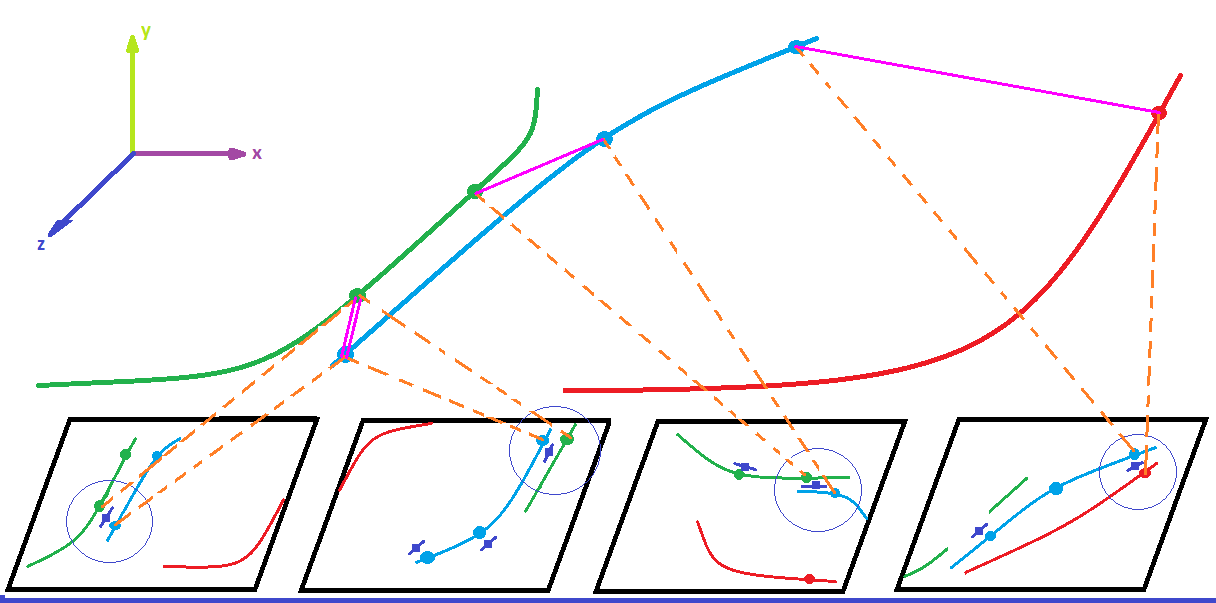
\includegraphics[width=0.75\linewidth]{figs/master-figure.png}} &
		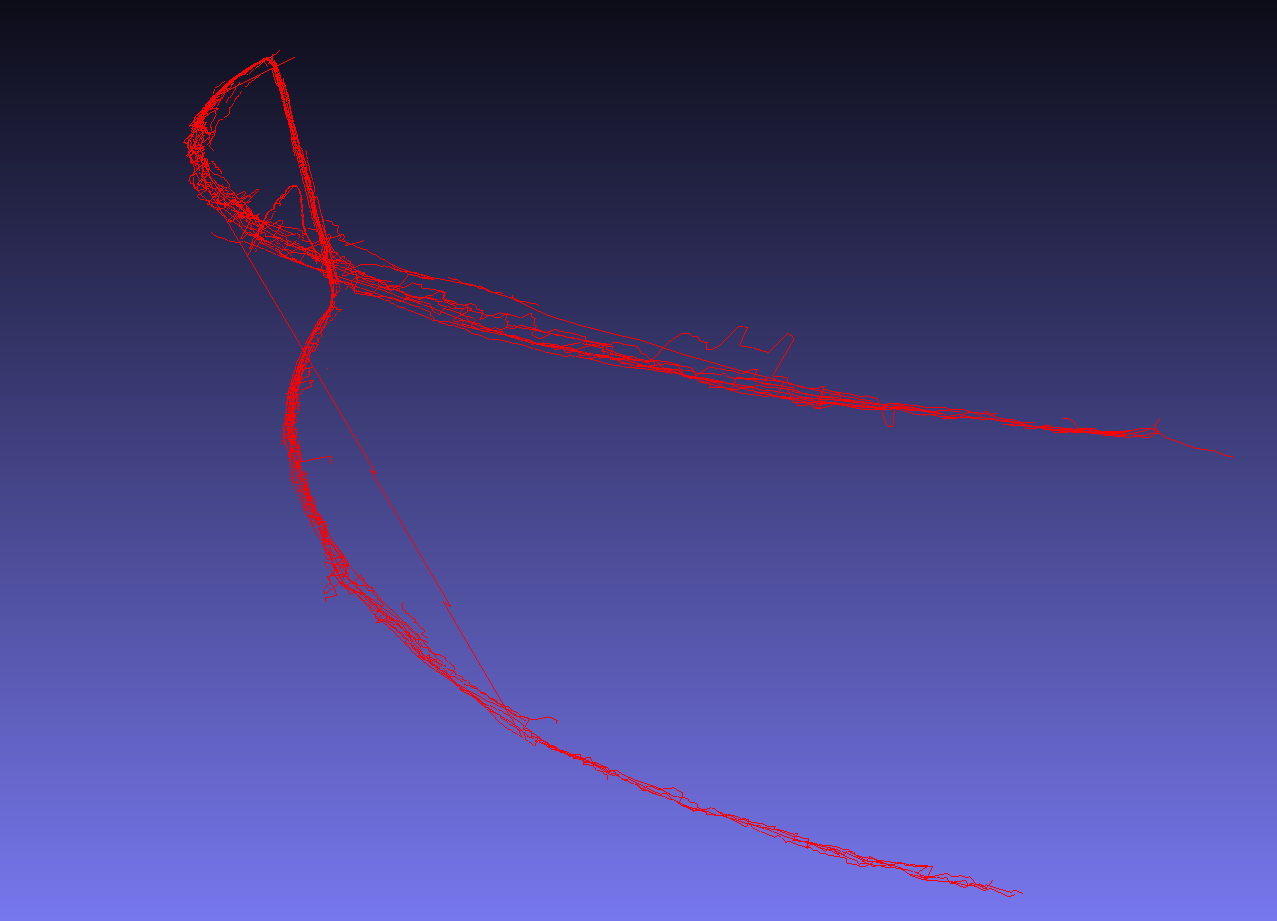
\includegraphics[width=0.2\linewidth]{figs/cluster32-2.png}\\
		&
		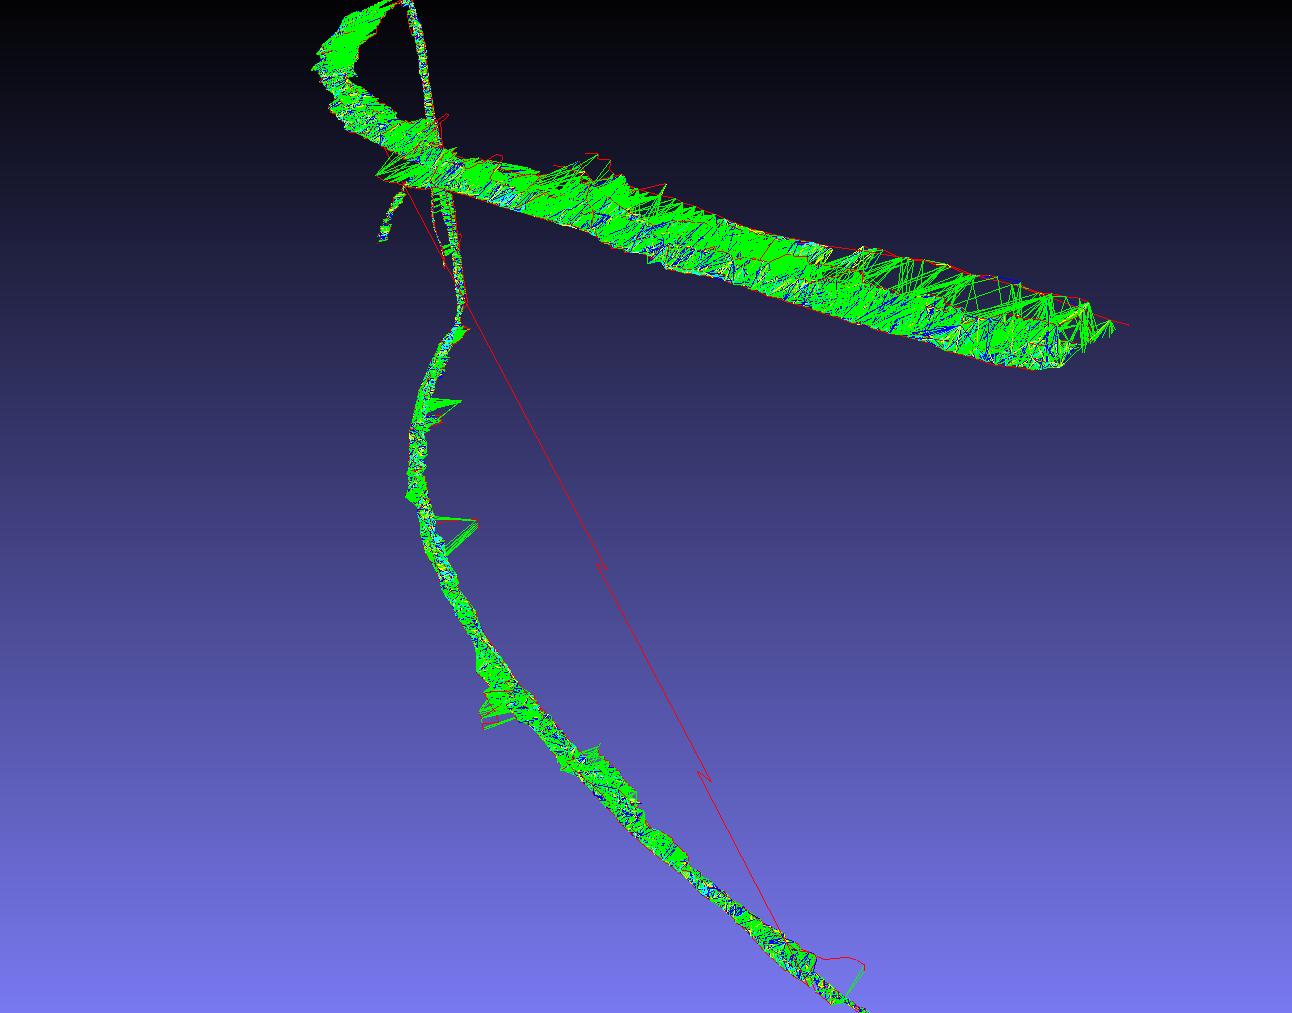
\includegraphics[width=0.2\linewidth]{figs/cluster32-corr2.png} \\
	\end{tabular}
	%\vspace{-0.3cm}
	\caption{\small The four bottlenecks of
		Fig.~\ref{fig:issues:remaining} are resolved by integration of
		information/cues from all views. (a) The shared supporting edges, which are marked with circles, create the purple links between the corresponding samples of the 3D curves. These purple bonds will then be used to pull the redundant segments together and reorganize the 3D model into a clean 3D graph. Observe how the determination of common	image support can identify portions of the green and blue curves as identical	while differentiating the red one as distinct. A real example for a bundle of related curves is shown in (b) and the links among their edges in (c).
	}
	%   based on which 3D information with a
	%   common cause can be integrated, leading to a four-stage process of $(i)$
	%   establishing the links as pictured above, $(ii)$ identifying portions of 3D
	%   curves which arise from the same source, Fig~\ref{fig:overlap:masks}, $(iii)$
	%   precise localization for 3D curves with a common cause,
	%   Fig~\ref{fig:graph:organization}a, (iv) Topological merging of these
	%   segments, leading to a topological graph of 3D curve segments,
	%   Fig~\ref{fig:graph:organization}e.}\label{fig:master:figure}
\end{figure}

%\vspace{-0.3cm}

\textbf{Multiview Curve-level Consistency Network:}
The identification of 3D edges sharing 2D edges leads to
high recall operating point with many false links due to accidental alignment of
edge support. False positives can be reduced without affecting high
recall by employing a notion of curve context for each 3D edgel: a link
between two 3D edgels based on a supporting 2D edgel is more effective if
the respective neighbors of the underlying 3D edge on the underlying 3D curve
are also linked. 

The curve context idea requires establishing new pairwise links between 3D
curves using MLN, when there are a sufficient number of links with
$\phi_{ij}>\tau_{\epsilon}$ between their constituent 3D edges (in our
implementation, $\tau_{\epsilon}=3$ and we require 5 such edges or more). The
linking of 3D curves is represented by the Multiview Curve-level Consistency
network (MCCN), a graph whose nodes are the 3D curves $\Gama_j$ and the edges
represent the presence of high-weight 3D edge links between these 3D curves. The
\mccn graph allows for a clustering of 3D curves by finding connected
components; and once a link is established between two curves, there is a high
likelihood of their edges corresponding in a regularized fashion, thus
fewer common supporting 2D edges are required to establish a link between all
their constituent 3D edges. This fact is used to perform gap filling, since even
no edge support is acceptable to fill in small gaps and create a continuous and
regularized correspondence if both neighbors of the gap are connected (see
pseudocode in Supplementary Materials for details). The two stages in
tandem, \ie, high recall linking of 3D edges and use of curve context to reduce
false positives leads to high recall and high precision, \textit{i.e.}, all the
3D edges which need to be related are related and very few outlier connections
remain.

\begin{figure}
	\captionsetup[subfigure]{labelformat=empty}
	\centering
	\begin{tabular}{cc}
		\multirow{2}[2]{*}[13mm]{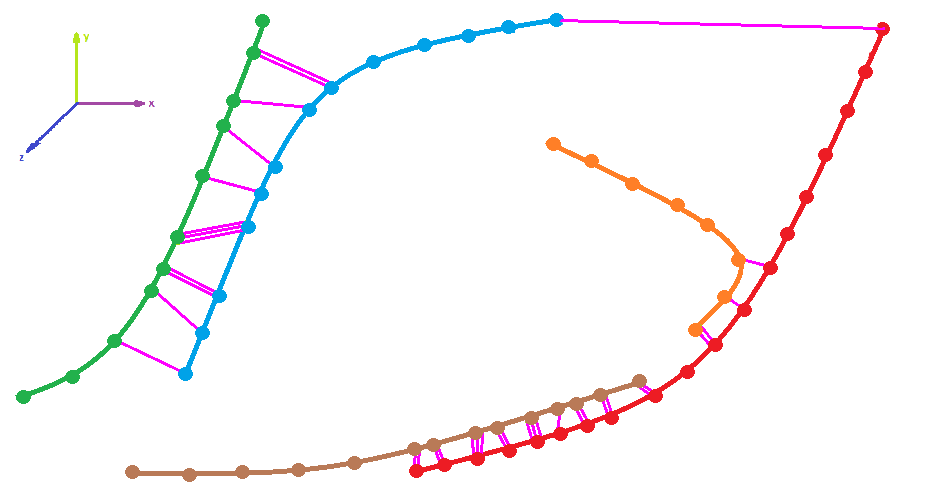
\includegraphics[width=0.55\linewidth]{figs/need-for-clusters.png}} &
		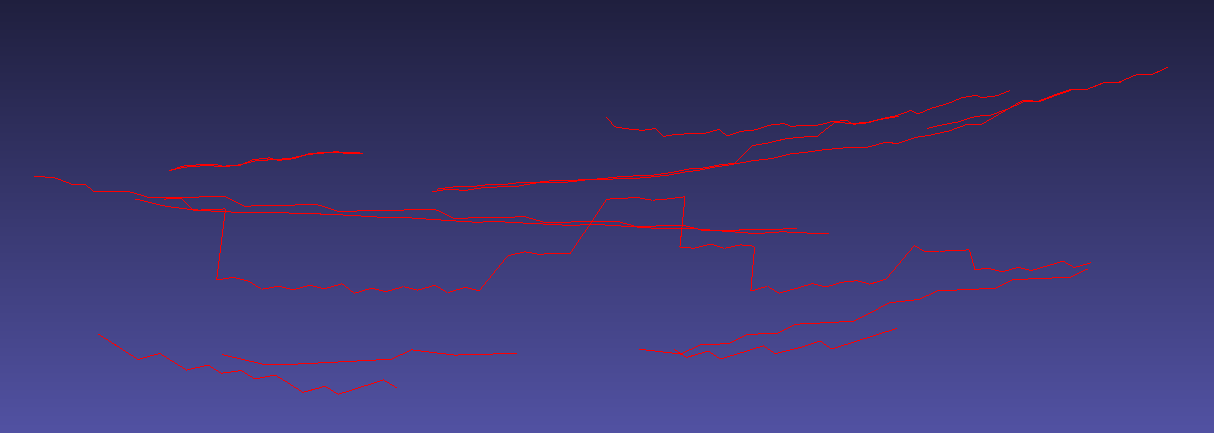
\includegraphics[width=0.45\linewidth]{figs/cluster7.png}\\
		&
		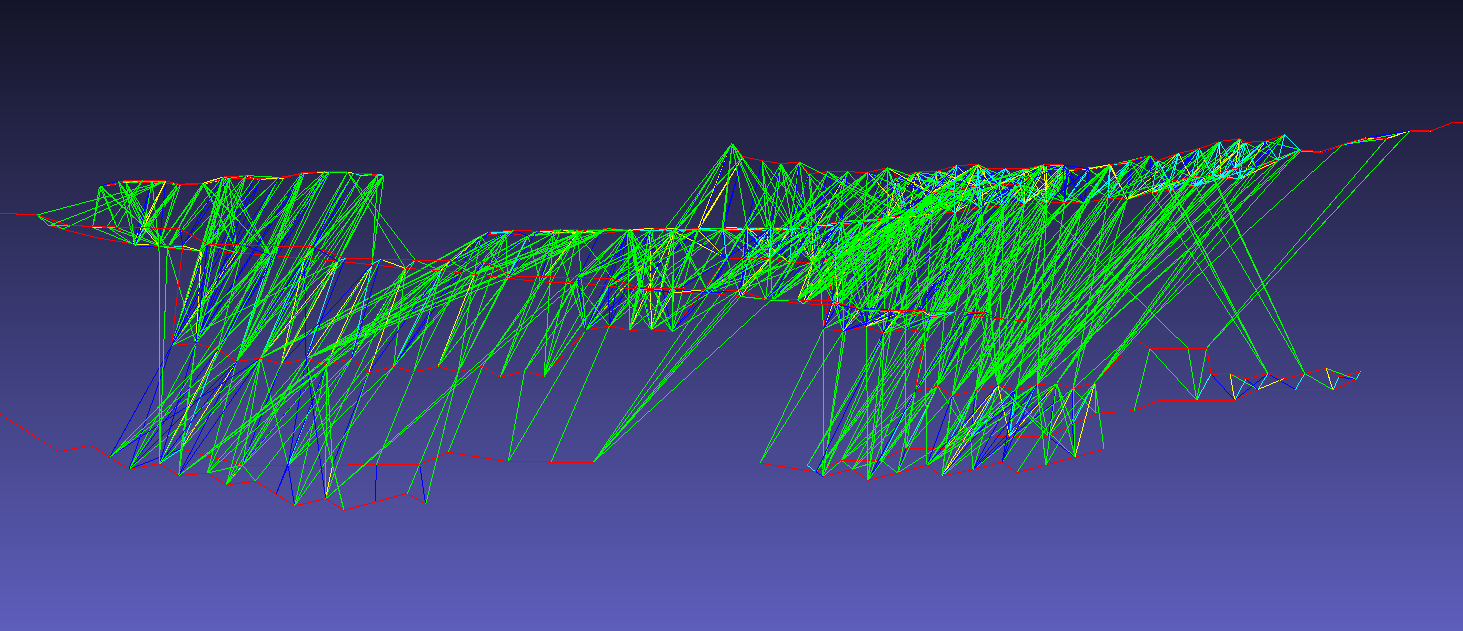
\includegraphics[width=0.45\linewidth]{figs/cluster7-corr.png}
		\\
	\end{tabular}
	%\ReduceBeforeCaptionfigspace
	\caption{\small 
		The correspondence between 3D edge samples is skewed along a curve, a direct indication that these links cannot be used as-is when averaging and fusing redundant curve reconstructions. Instead, each point is assumed to be in correspondence with the point closest to it on another overlapping curve, during the iterative averaging step. Observe that corrections can be partial along related
		curves.
	}
	\label{fig:overlap:masks}
\end{figure}

%\vspace{-0.3cm}

%The links between two 3D curves that are consistently overlapping according to
%evidence from multiple views form the so-called Multiview Curve-level
%Consistency Network, a graph defined as follows.
%\begin{definition}
%The Multiview Curve-level Consistency Network (MCCN) is a graph 
%\begin{equation}
%\text{\textit{MCCN}} = (S, L),
%\end{equation}
%where the vertices $S = \{1,\dots,K\}$ encode the set of 3D curves
%$\{\Gama_1,\dots,\Gama_K\}$ and $L$ is the link set defined below.
%\end{definition}
%\begin{definition}
%Let the set of so-called strong local links between curves $\Gama_i$ and
%$\Gama_j$ be defined as
%\begin{equation}
%S_{ij} \doteq \{(s,t) : \phi_{ij}(s,t) \geq \tau_{s}, \phi_{ij} \in
%\text{MLN}(\Gama_1,\dots,\Gama_K) \}.
%\end{equation}
%Then the set $L$ of the MCCN is defined as
%\begin{equation}
%L = \{(i,j) : |S_{ij}| \geq \tau_{sl}\}.
%\end{equation}
%\end{definition}
%\indraftnote{We can formulate L as an integral over alignment parameter, see
%rics notes}

%We cluster the 3D curves by computing the connected components of their MCCN.
%We then go back to local correspondences by filling-in short correspondence gaps
%of the MLN induced by the confidence gained by the curve-level consistency link.
%Further details are available in the form of a pseudocode in supplementary material.


\textbf{Integrating information across related edges:} 
The identification of a bundle of curves as arising from the same 3D source
implies that we can improve the geometric accuracy of this bundle by
allowing them to converge to a common solution. While this might appear
straightforward, 3D edges are not consistenly distributed along related curves,
yielding a skew in the correspondence of related samples,
Fig.~\ref{fig:overlap:masks}, sometimes not a one-to-one
correspondence, Fig.~\ref{fig:graph:organization}a. This argues for averaging 3D
curves and not 3D edge samples, which in turn requires finding a more
regularized alignment between the 3D curves, without gaps; we find each
curve samples's closest point on the other curve.

\begin{figure}[htbp]
	\begin{center}
		\centering
		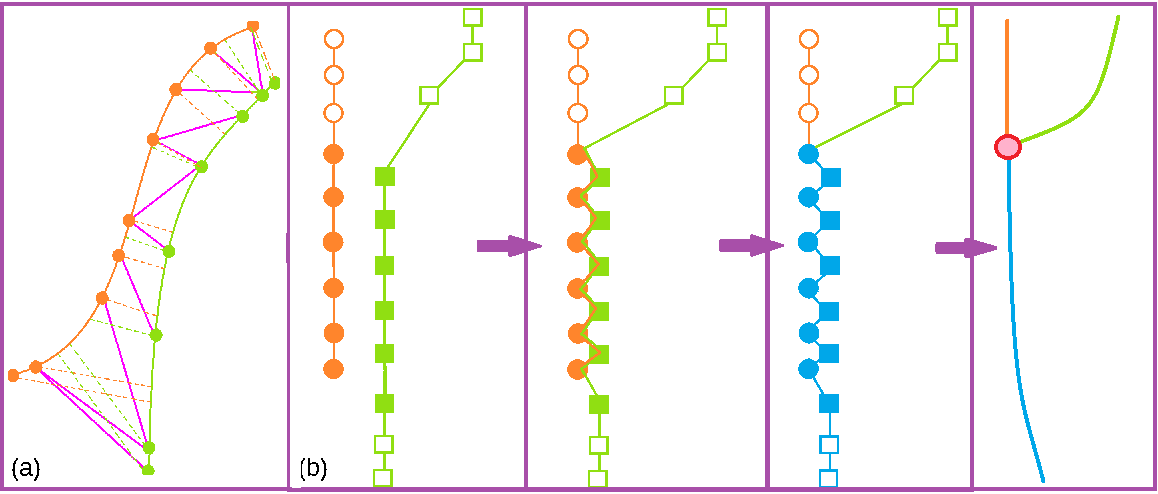
\includegraphics[width=0.86\linewidth]{figs/graph-organization-caption.pdf}
		%   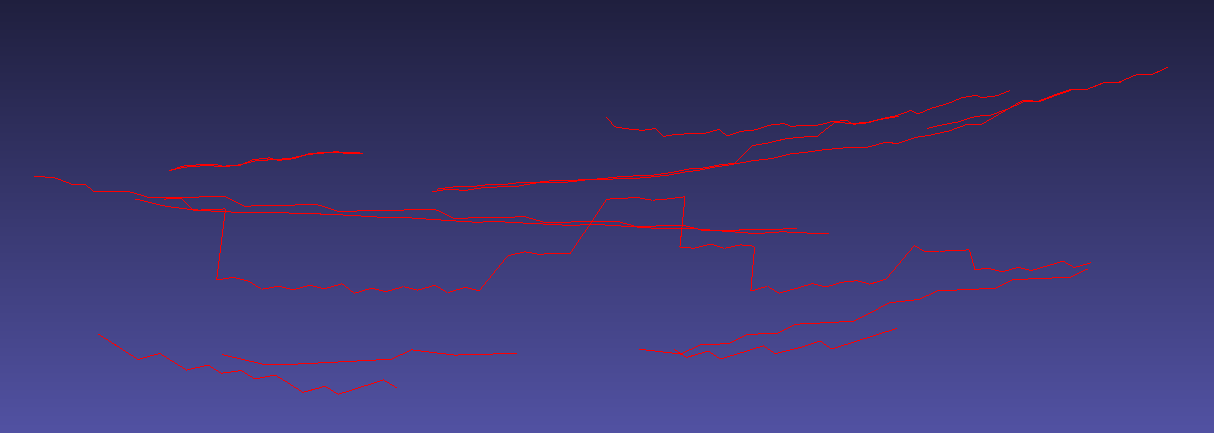
\includegraphics[width=0.32\linewidth]{figs/cluster7.png}
		%   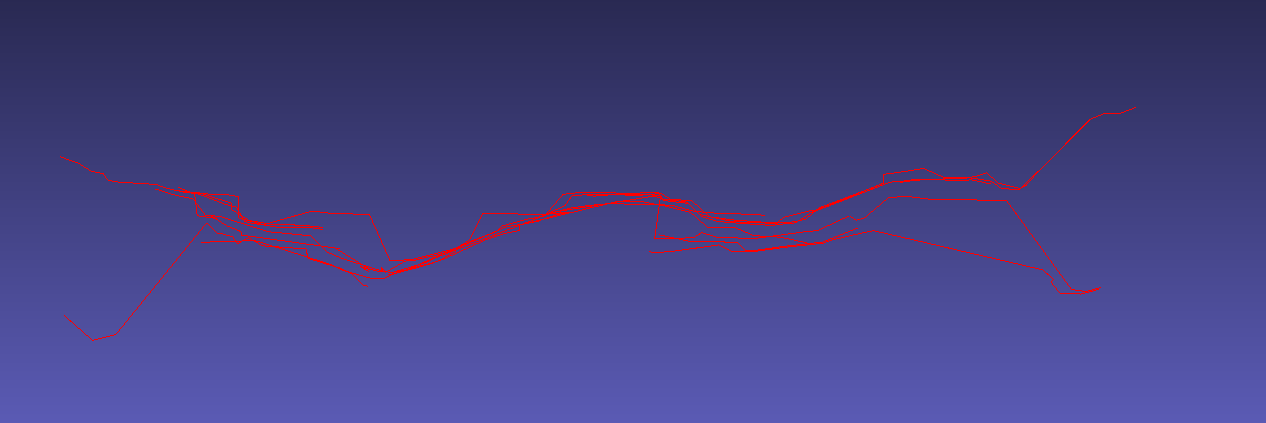
\includegraphics[width=0.32\linewidth]{figs/cluster7-after.png}
		%   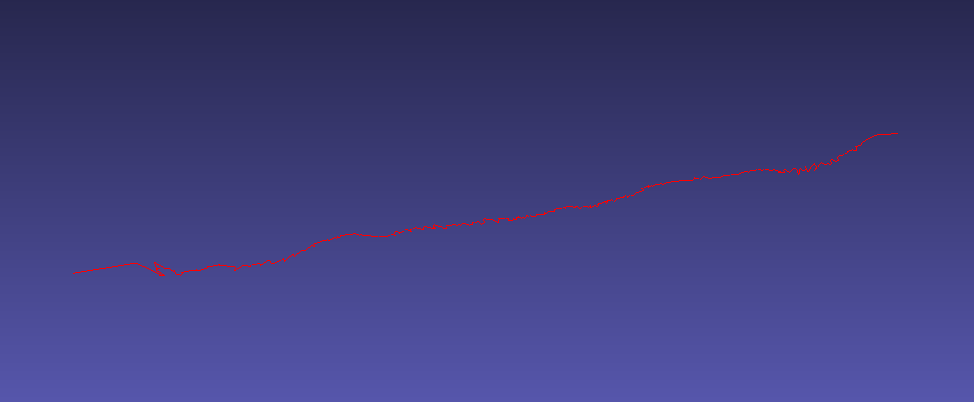
\includegraphics[width=0.32\linewidth]{figs/cluster7-merged.png}
		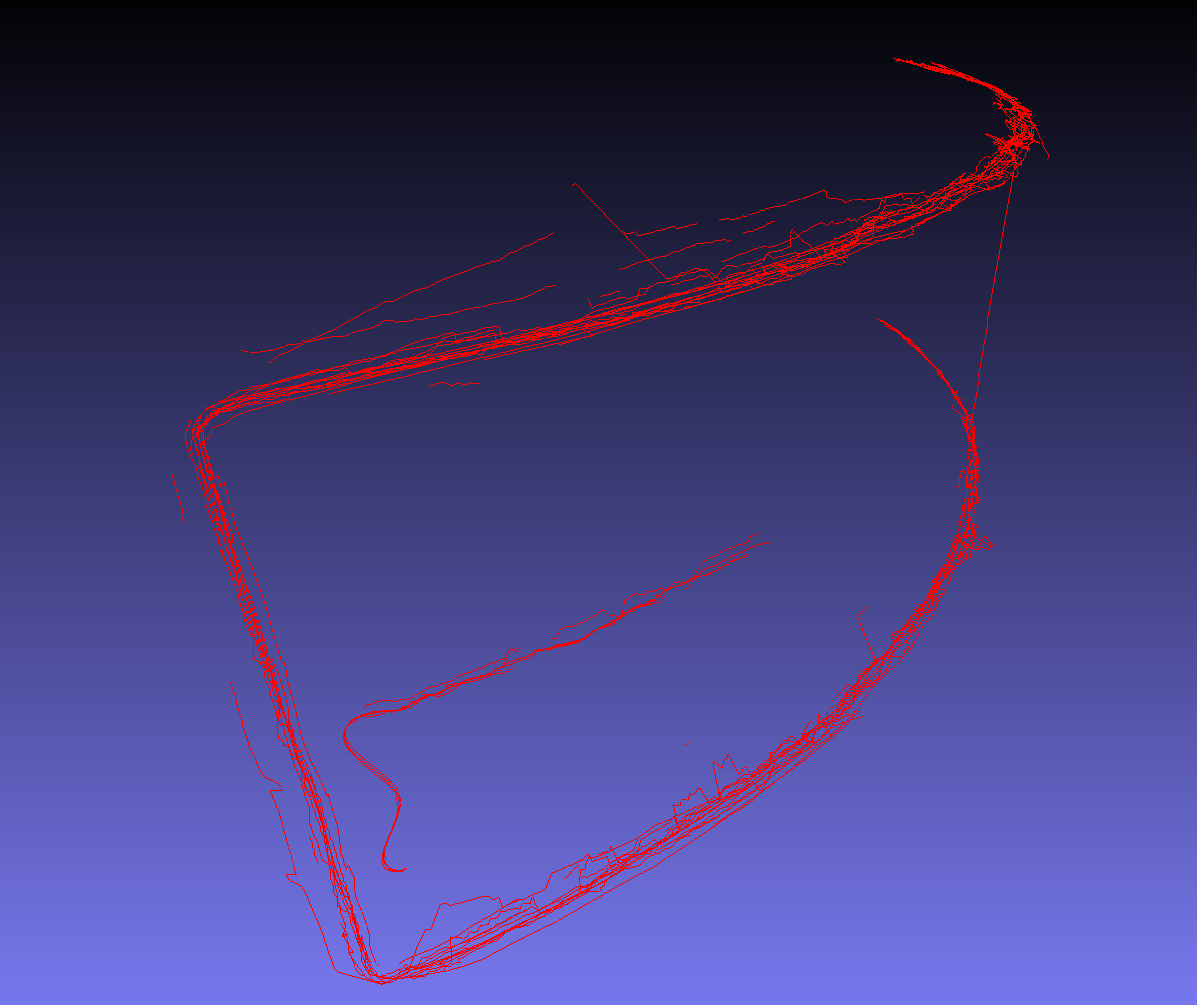
\includegraphics[height=2.8cm]{figs/cluster32-1.png}
		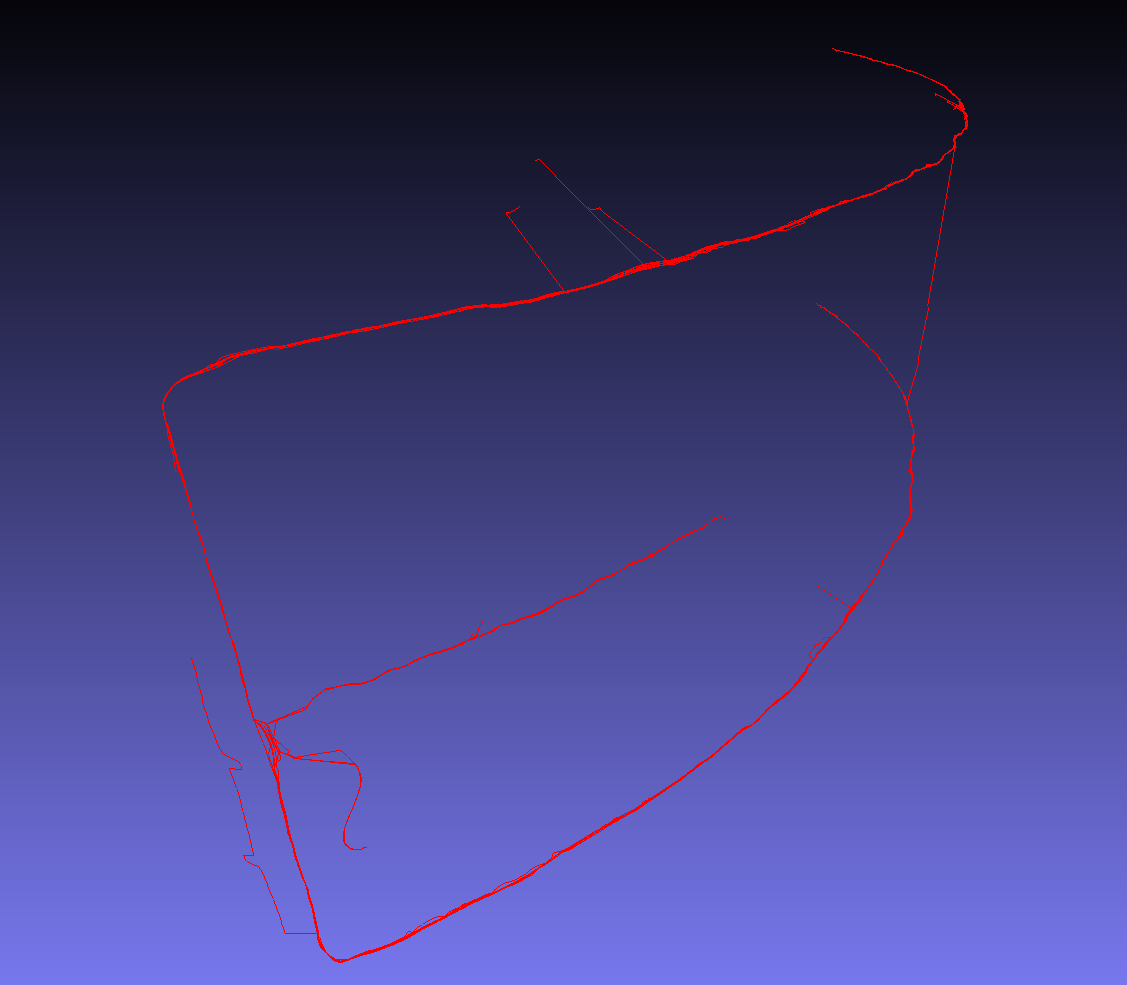
\includegraphics[height=2.8cm]{figs/cluster32-after1.png}
		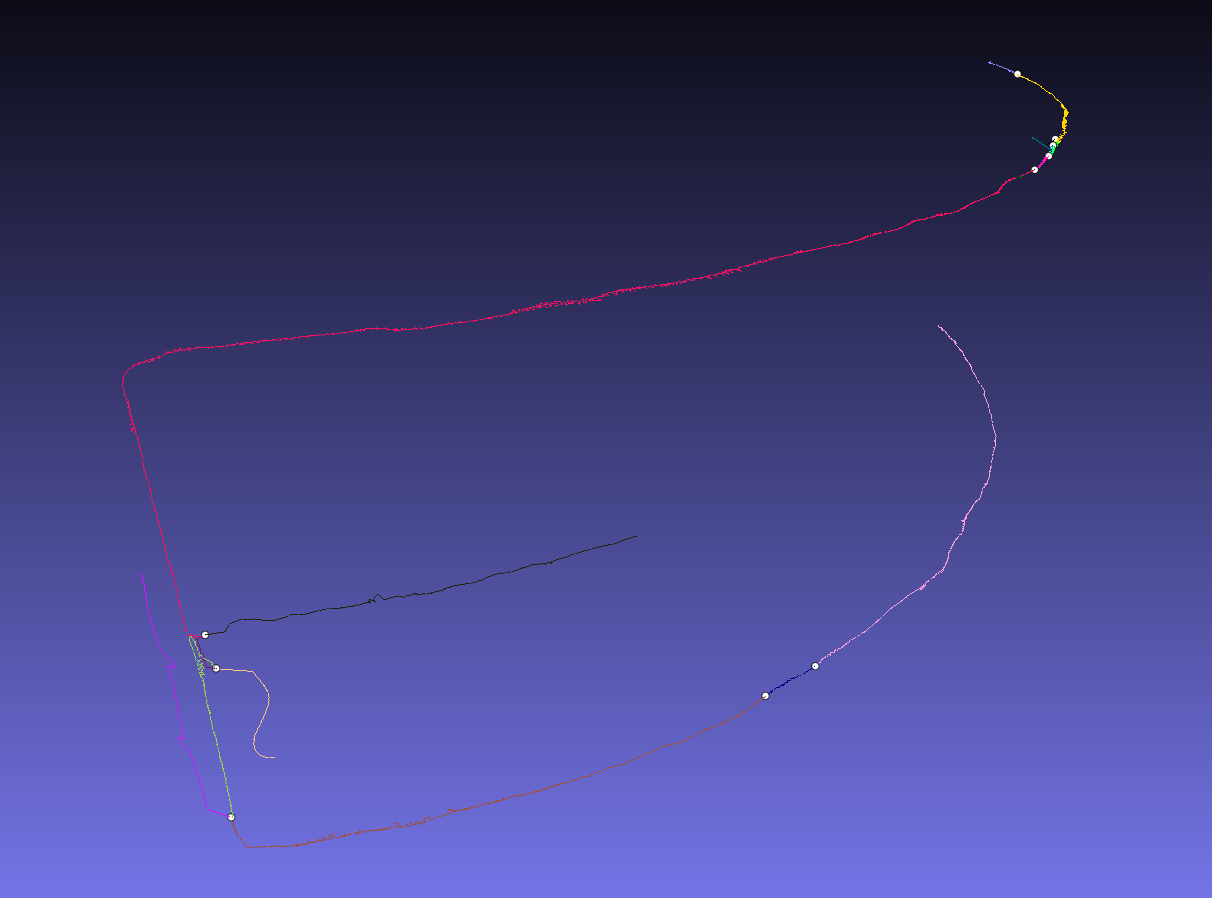
\includegraphics[height=2.8cm]{figs/cluster32-merged1.png}
		%   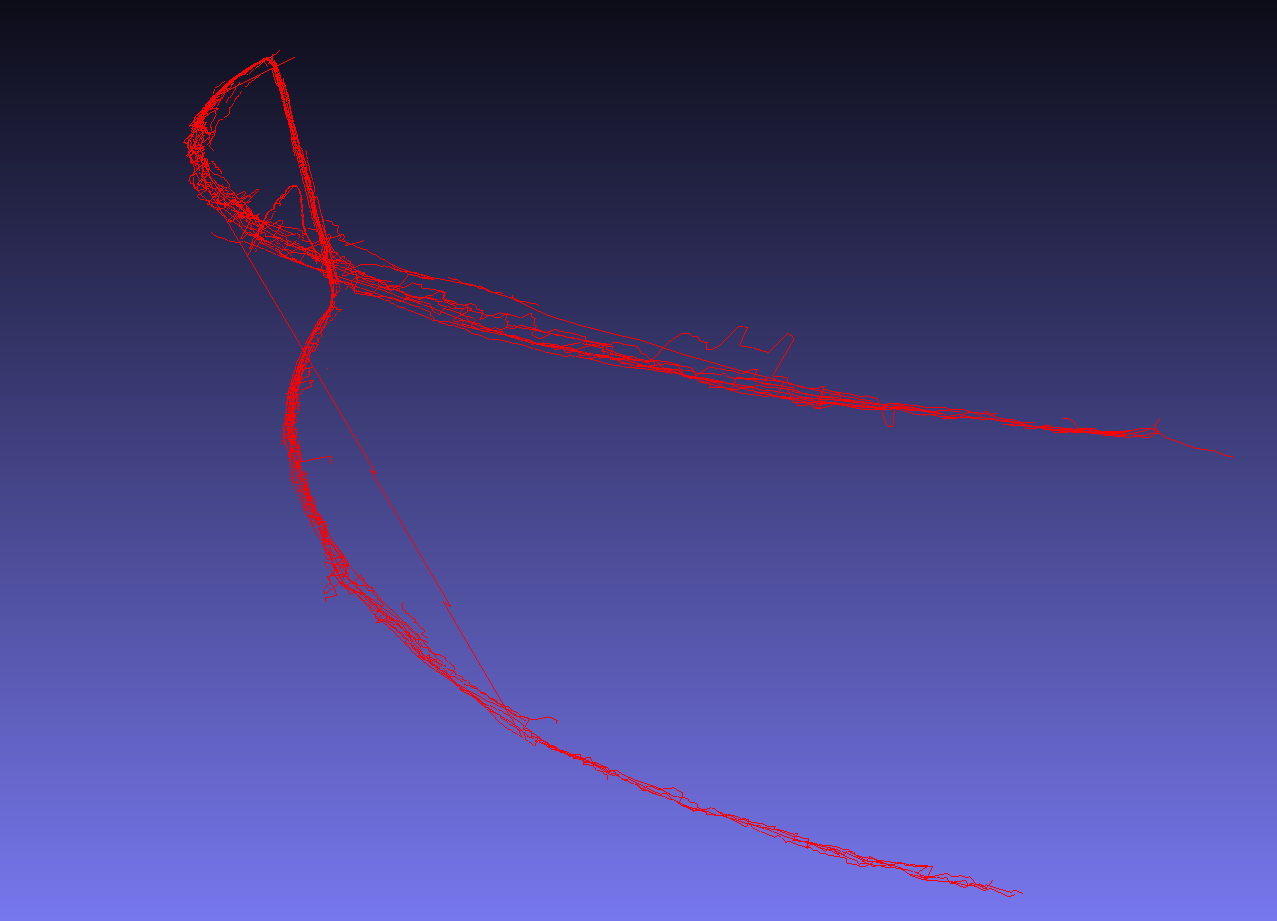
\includegraphics[width=0.32\linewidth]{figs/cluster32-2.png}
		%   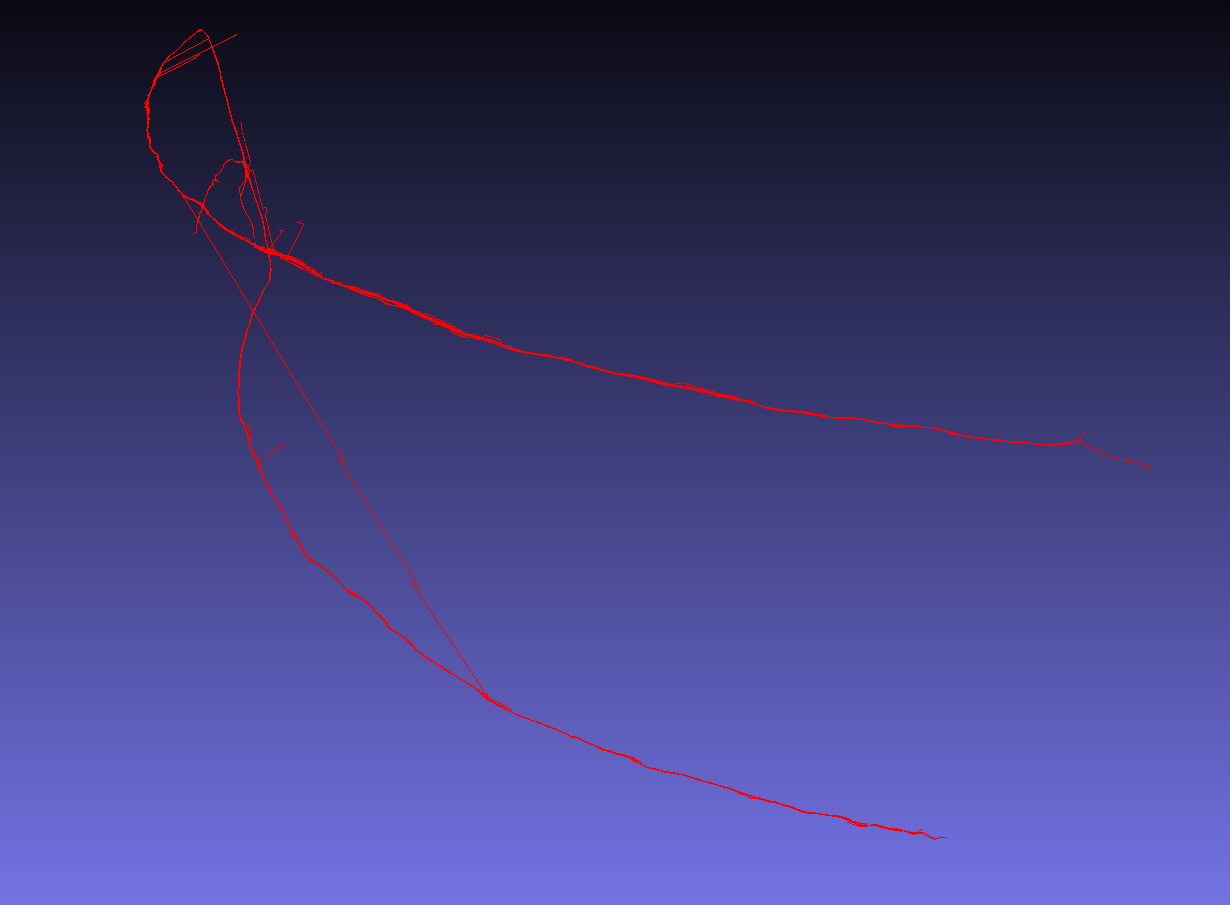
\includegraphics[width=0.32\linewidth]{figs/cluster32-after2.png}
		%   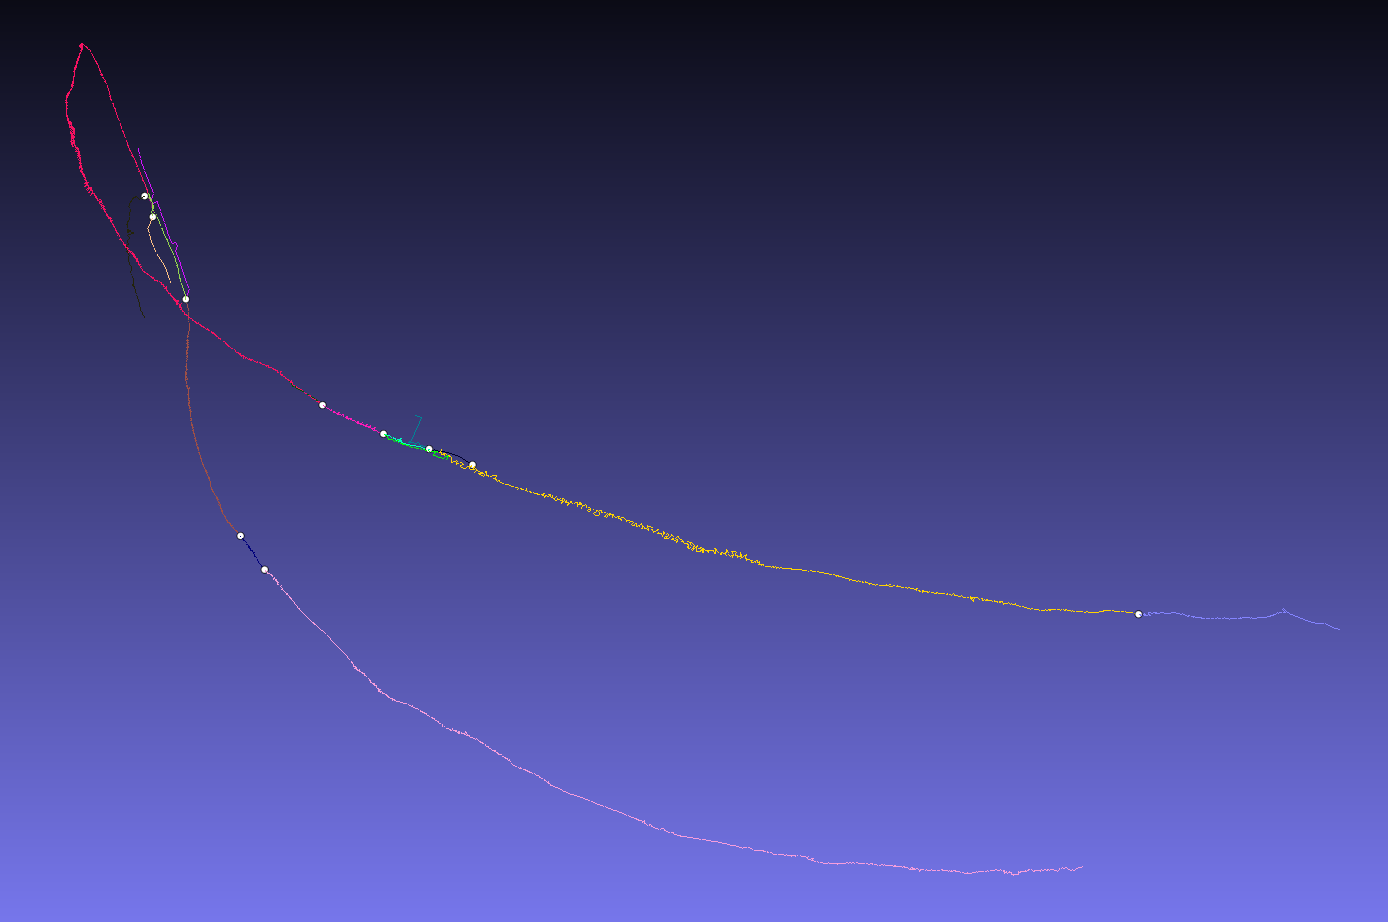
\includegraphics[width=0.32\linewidth]{figs/cluster32-merged2.png}
	\end{center}
	\caption{\small (a) A schematic of sample correspondence along two related 3D
		curves, showing skewed correspondences that may not be one-to-one. (b) A
		sketch of how two curves are integrated. Bottom row: a real case.
	}
	\label{fig:graph:organization}
\end{figure}

When post averaging a sample with its closest points on related curves, the
order of resulting averaged samples is not clear.  The order should be inferred
from the underlying curves, but this information can be
conflicting, unless the distance between two curves is substantially smaller
than the sampling distance along the curves. This requires
first updating each curve's geometry separately and iteratively, without
merging curves until after convergence,
Fig.~\ref{fig:graph:organization}d. This also improves the correspondence of
samples at each iteration, as the closest points are continuously updated. 

At each stage, the iterative averaging process simply replaces each 3D edge
sample with the average of all closest points on curves related to it,
Fig~\ref{fig:graph:organization}b--d. This can be formulated
as evolving all 3D curves by averaging along the \mccn using closest points.
Formally, each $\Gama_i$ is evolved according to
%{\small
\begin{equation}
\frac{\partial\Gama_i}{\partial t}(s) = \alpha 
\avg_{\substack{(i,j)\in L\\ (\Gama_i, \Gama_j) \in \text{ \textsc{mccn}}}}
\{\Gama_j(r) : \Gama_j(r) = \text{cp}_j(\Gama_i(s)) \},
\end{equation}%}
where $\text{cp}_i(\mathbf p)$ is the closest point in $\Gama_i$ to $\mathbf p$ and $L$ is the link set defined as follows:
Let the set $S_{ij}$ of so-called strong local links between curves $\Gama_i$ and
$\Gama_j$ be
\begin{equation}
S_{ij} \doteq \{(s,t) : \phi_{ij}(s,t) \geq \tau_{\epsilon}, \phi_{ij} \in
\text{MLN}(\Gama_1,\dots,\Gama_K) \}.
\end{equation}
Then the set $L$ of the \mccn is defined as
\begin{equation}
L \doteq \{(i,j) : |S_{ij}| \geq \tau_{sl}\}.
\end{equation}
In practice, the averaging is robust and $\alpha$ is chosen such that in
one step we move to the average.

\textbf{3D Curve Drawing Graph:}
Once all related curves have converged, they can be merged into single curves,
separated by junctions where 3 or more curves meet. The order along the
resulting curve is also dictated by closest points: The immediate neighbors of
any averaged 3D edge are the two closest 3D edges to it among all
converged 3D edges in a given \mccn cluster.

This where junctions naturally arise: as two distinct curves may merge along one
portion they may diverge at one point, leaving two remaining, non-related
subsegments behind, Fig~\ref{fig:graph:organization}e.  This is a \emph{junction
node} relating three or more curve segments, and its detection is done using the
\emph{merging primitives}, whose complete set are shown in
Fig.~\ref{fig:junction:topology}. The intuition is this: a
complex merging problem along the full length of two 3D curves actually consists
of smaller, simpler and independent merging operations between different
segments of each curve. A full merging problem between two complete
curves can be expressed as a permutation of any number of simpler merging
primitives. These primitives were worked out systematically to serve as the
basic building blocks capable of constructing \emph{all possible configurations}
of our merging problem. 

%in this way, the set of these primitives is not an
%arbitrary heuristic but rather is a complete set of basic operations capable of
%breaking any merging problem into smaller chunks.

%\vspace{-0.8cm}

\begin{figure}[h]
	\begin{center}
		\centering
		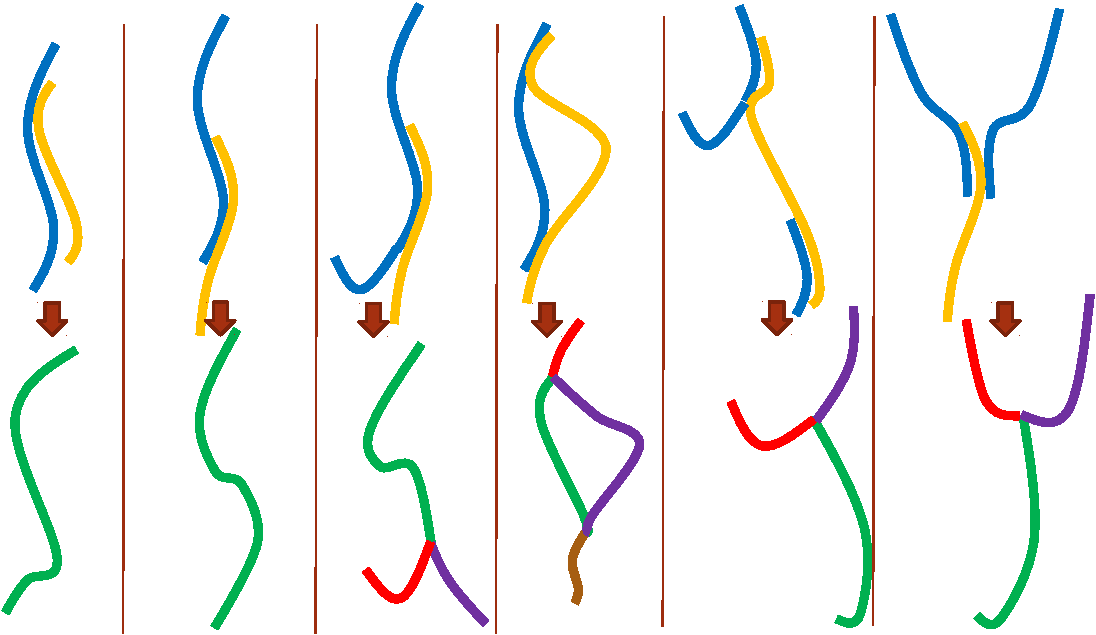
\includegraphics[width=0.4\linewidth]{figs/topology.pdf}
	\end{center}
	\caption{\small The complete set of merging primitives, which were
  systematically worked out to cover all possible merging topologies between a
pair of curves whose overlap regions are computedbeforehand. We claim that any
configuration of overlap between two curves can be broken down into a series of
these primitives along the length of one of the curves. The 5th primitive is
representative of a ``bridge'' situation, where the connection at either end of
the yellow curve can be any one of the first four cases shown, and 6th primitive
is representative of a situation where only one end of the yellow curve connects
to multiple existing curves, but not necessarily just two.}
	\label{fig:junction:topology}
\end{figure}

After iterative averaging, all resulting curves in any given cluster
are processed in a pairwise fashion using these primitives: initialize the 3D
graph with the longest curve in the cluster, and merge every curve in
the cluster one by one into this graph. At each step, any number of these
merging primitives arise and are handled appropriately. This process outputs the
Multiview Curve Drawing Graph (MDG), which consists of multiple disconnected 3D
graphs, one for each 3D curve cluster in the MCCN. The nodes of each graph are
the junctions (with curve endpoints) and the links are curve fragment
geometries. This structure is the final 3D curve drawing.

\begin{figure}[h!]
\begin{center}
  \begin{draft} 
  [orig chair images here]
  \end{draft}
%   \includegraphics[width=1.0\linewidth]{figs/3d-curve-sketch/system-diagram.eps}
    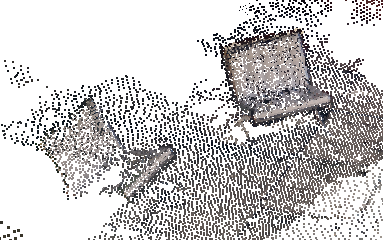
\includegraphics[width=0.45\linewidth]{figs/pavilion-midday-pmvs-1.png}
    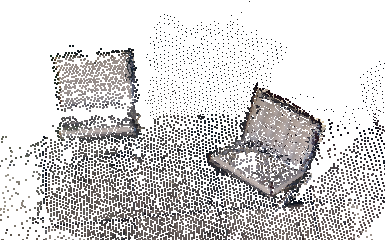
\includegraphics[width=0.45\linewidth]{figs/pavilion-midday-pmvs-2.png}\\
    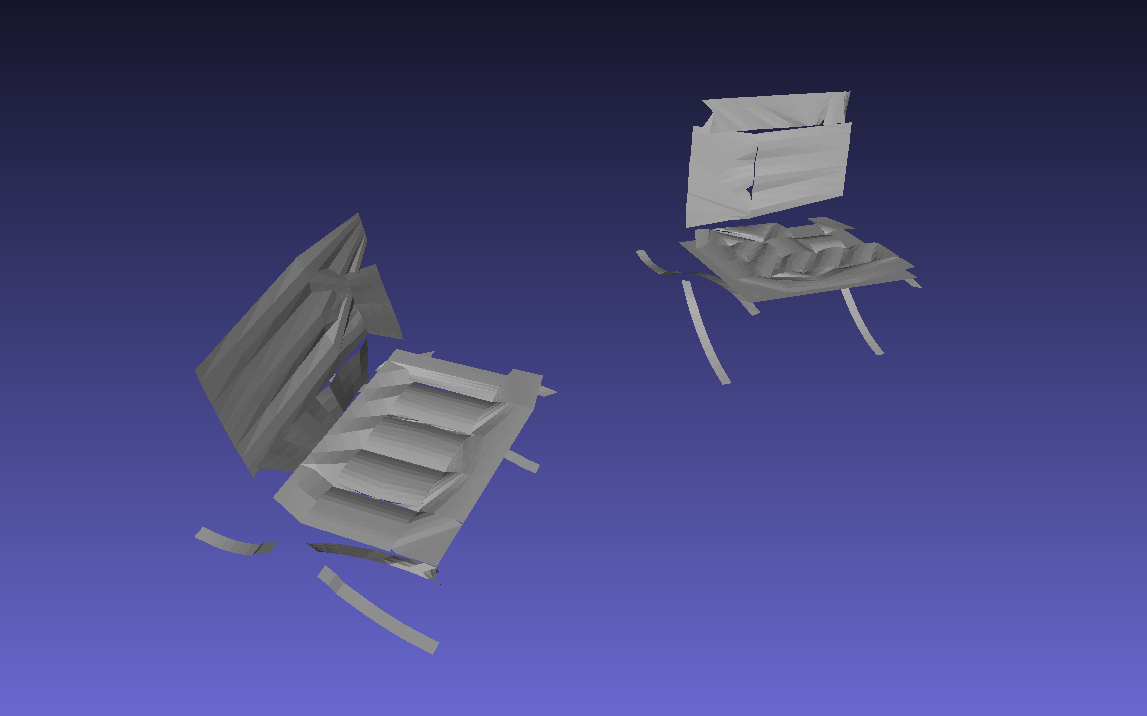
\includegraphics[width=0.45\linewidth]{figs/pavilion-loft2sm.png}
    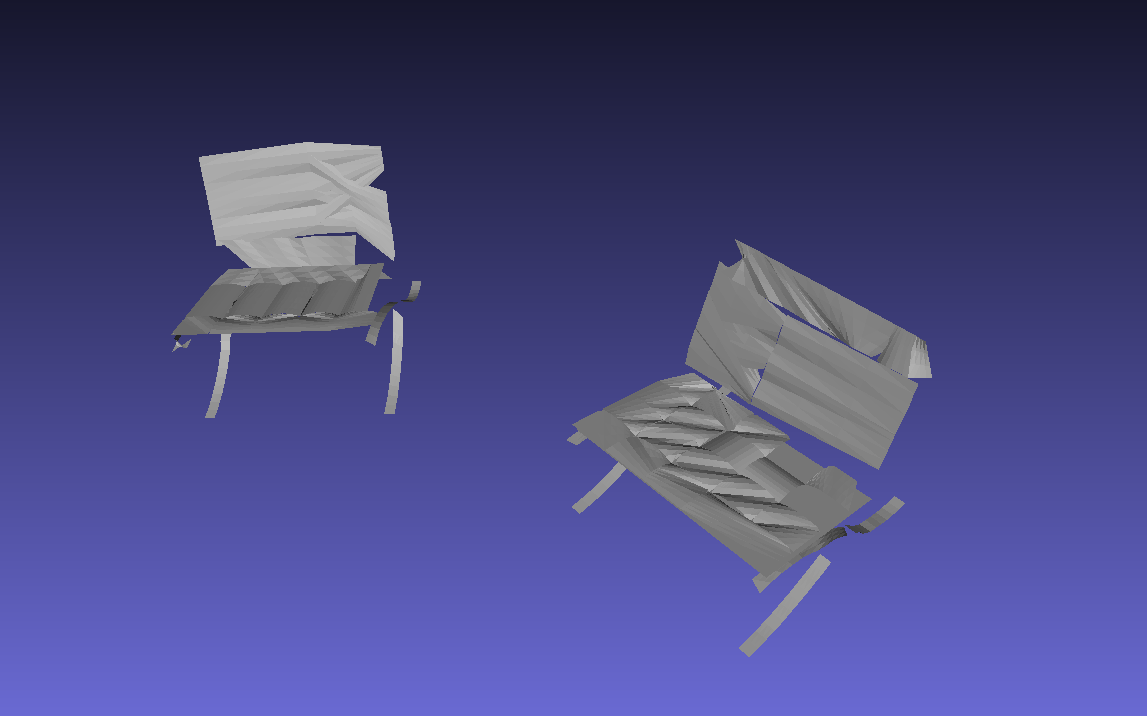
\includegraphics[width=0.45\linewidth]{figs/pavilion-loft1sm.png}
\end{center}
\vspace{-0.7truecm}
   \caption{%
     \textbf{Acima:} reconstru��o 3D tradicional por \emph{structure from motion} de
     pontos. \textbf{Abaixo:}
     Reconstru��o 3D de superf�cies pasando-se por
     curvas~\cite{Usumezbas:Fabbri:Kimia:CVPR:2017} em objetos dif�ceis de
     reconstruir usando pontos de interesse ou apenas intensidade. Esta
     reconstru��o usa apenas informa��o de curvas, sem nenhum sombreadmento,
     sendo extremamente robusta a grande varia��es de ilumina��o. Pretende-se, neste projeto,
     usar um algoritmo de agrupamento dos fragmentos de superf�cie mais
     elaborado (um avan�o na �ltima caixa listada na
     Figura~\ref{fig:system:diagram}, bem como usar a informa��o temporal em v�deo para reconstruir
     contornos de oclus�o (siluetas locais), uma t�cnica com uma teoria muito
     promissora~\cite{Giblin:Motion:Book} que nunca foi posta em
     pr�tica pois a tecnologia de reconstru��o 3D por curvas n�o era desenvolvida.
     Este �ltimo seria um avan�o significativo na pen�ltima caixa da
     Figura~\ref{fig:system:diagram}.
   }\label{fig:chairs}
\end{figure}



\subsection{Other objectives}
\begin{itemize}
\item Help with the book to be published
\item Take part in helping teach a graduate-level course.
\end{itemize}


\section{Methodology}

\section{Results}

\section{Cronograma das Atividades}
A tabela abaixo mostra o cronograma para as principais atividades descritas. Para a
execu��o deste projeto, o per�odo foi dividido em etapas trimestrais.
\begin{center}
\begin{tabular} {||r|c|c|c|c||}
\hline
\textbf{Stages (trimesters)} & 1 & 2 & 3 & 4 \\
\hline
Reproduce 3D Curve Sketch System& X &  & & \\
\hline
Reproduce 3D Curve Drawing System& X & X & & \\
\hline
Reproduce 3D Lofting System &   & X &  & \\
\hline
Build graphs for surface merging& X & X & X & \\
\hline
Large scale expermients&   &   & & X\\
\hline
Write Software & X & X & X & X\\
\hline
Publish Open Source Software &  &  & X & X \\
\hline
Publications &  & X & X& X\\
\hline
\end{tabular}
\end{center}


\nocite{Fabbri:2002}
\addcontentsline{toc}{section}{Refer\^{e}ncias}
\bibliographystyle{ieeetr}
\bibliography{personal,strings,shading,multiview,motion,Kimia,catagorization,edge-linking,deformable,medical,graphics,active-contours,texture,imaging,tracking,shape-papers,bib-header,video,math-books,math,psych-books,metric,edge,leymarie_pami_scaffold,vision-books,vision,nn-search,multidimscaling,psychophysics,indexing,segmentation,image-databases,shape-matching,neuro,skeleton,skeleton2D,aspect-graphs,recognition,surface-networks,ridge,proceedings,perceptual-grouping,continuation,graph-matching-2,cooper}
%\input{paper.bbl}
%
% Assinaturas:
%\newpage
%\ \\\vspace{7cm}
%\center $\overline{\ \ \ Ricardo\ Fabbri\ \ \ }$
%\ \\\vspace{4cm}
%\center $\overline{\ \ \ Luciano\ da\ Fontoura\ Costa\ \ \ }$
\end{document}
